\chapter{Stock returns over the FOMC Cycle Revisited }


\section{The FOMC cycle}

The FOMC meets approximately every eight weeks during the year,  resulting in an FOMC cycle time of approximately 7 weeks (excluding weekends) most of the time since a year has 52 weeks. The authors, therefore, define FOMC cycle time week dummy variables for week 0 as days -1 to 3, week 1 as days 4 to 8, and week 6 as days 29 to 33. Worth mentioning is that the authors drop 3 days, which would be in FOMC cycle week 7 from their investigation, and that the number of available data points decreases for FOMC dummies (meaning 920 days in week 0,  924 days in week 2,  831 days in week 4,  120 days in week 6 for the relevant timespan from 1994 to 2016).

\label{cies19_fig2}
\begin{figure}[h]
    \centering
    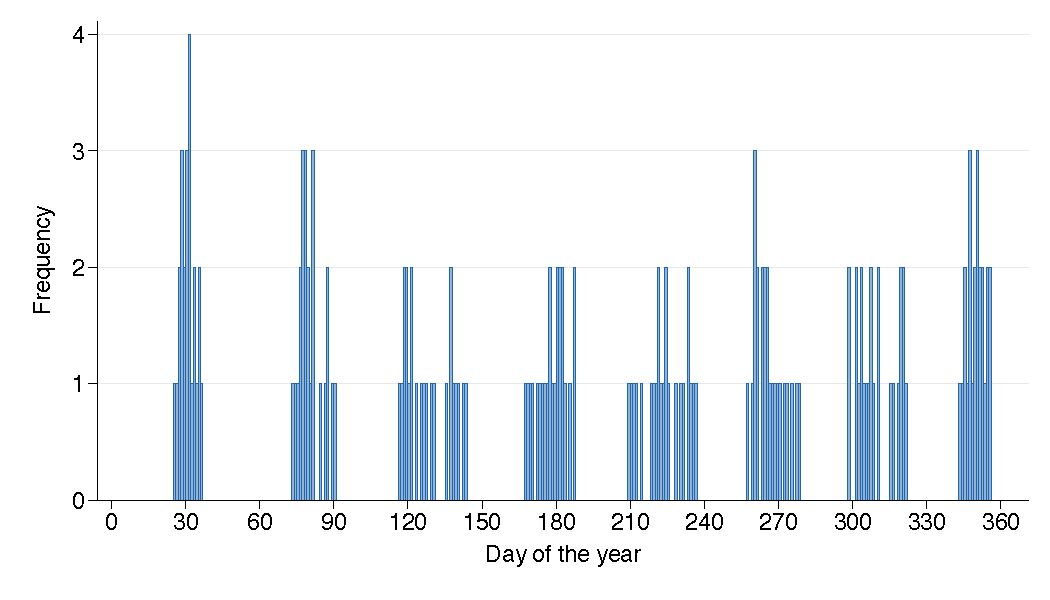
\includegraphics[width=0.75\textwidth]{figures/cies19/fig2}
    \caption{Frequency of FOMC meetings during the year from 1994 to 2016 \parencite{cieslak_stock_2019}}
\end{figure}


\section{Institutional Setting}

The Federal Reserve System is comprised of the Board of Governors, 12 Federal Reserve Banks, and the FOMC. The FOMC's 12 members are responsible for implementing monetary policy to achieve macroeconomic goals, such as adjusting federal fund rates and conducting large-scale purchases of treasury securities and federal agency-issued or guaranteed securities since the 2008 financial crisis as policy tools to lower long-term interest rates, ensuring the functioning of the U.S. economy.\footnote{\url{https://www.federalreserve.gov/aboutthefed.htm}}. 

\section{FOMC Data}

The FOMC publishes detailed records of its meeting proceedings on the Federal Reserve's webpage\footnote{\url{https://www.federalreserve.gov/monetarypolicy/fomccalendars.htm}}.  
The transcripts have been produced by the FOMC Secretariat shortly after every meeting since the year 1994.
The meeting participants have the opportunity to review the transcripts for accuracy within the subsequent weeks. 
These transcripts are available on the Federal Reserves webpage and contain a very small amount of confidential information that may be deleted. 
The FOMC also issues a policy statement after each meeting,  summarizing the economic outlook and their policy decisions. 
The Chairman holds press briefings to discuss policy decisions and economic projections. 
The minutes of the meetings are released three weeks after every regular meeting, and the meeting transcripts are accessible for up to five years after the meeting.

\section{Statistical Analysis}

\subsection{MLR model}

One relevant multiple linear regression (MLR) model with dummy variables for even FOMC cycle weeks as in \parencite{cieslak_stock_2019} can be defined as:
\begin{equation}
	ex1_{i}=\beta_{0}+D_0*\gamma_{1}+D_1*\gamma_{2}+\epsilon_i
\end{equation}
where
\begin{equation}
    D_0=
    \begin{cases}
      1, & \text{If in week 0 of FOMC cycle time}\\
      0, & \text{Otherwise}
    \end{cases}
\end{equation}
is a function equal to 1 if the FOMC cycle dummy is in week 0,
\begin{equation}
    D_1=
    \begin{cases}
      1, & \text{If in week 2,4 or 6 of FOMC cycle time. } \\
      0, & \text{Otherwise}
    \end{cases}
\end{equation}
is a function equal to 1 if the FOMC cycle dummy is in week 2,  4 or 6,
$ {ex1_{i}} $ are the 1-day risk-free excess returns on stocks,
$ { \hat{\beta_{0}} } $ is the OLS-estimated intercept,
$ { \hat{\gamma_{1}}, \hat{\gamma_{2}} } $   and
$ { \epsilon_i \; \sim \; i.i.d.  \; \mathcal{N}\left(0, \sigma^2 \right) } $
are independent identically distributed OLS-estimated standard errors. 
The OLS-estimated parameter $ {\hat{\gamma_{1}}} $ is of more importance with subject to the probability of target changes between meetings.

\subsection{FOMC dummies}

The R Code in \texttt{generate\_fomc\_dummies\_cycle\_dummies.R} (see Appendix)
generates FOMC week dummy variables by using the \texttt{"FOMC\_Cycle\_dates\_1994\_nov2023.xlsx"} file containing FOMC meeting dates for later estimation of the influence of the FOMC cycle on excess stock returns.

\subsection{Data Preprocessing}

The analysis commences with the importation and organization of two datasets. 
The first dataset, identified as \texttt{fomc\_data}, is loaded from the file \texttt{fomc\_week\_dummies\_1994\_nov2023.csv}. 
This dataset includes information related to FOMC week dummies spanning from November 1994 to November 2023. The data is sorted by date, and the sorted dataset is then saved as \texttt{d:fomc\_data}, thereby replacing any pre-existing file.

Following this, the second dataset, labeled as \texttt{us\_returns\_data}, is imported from the file \texttt{us\_returns\_df\_1994\_oct2023.csv}. This dataset contains information regarding Fama-French factors for the U.S. market, covering the period from October 1994 to October 2023. Similar to the first dataset, it undergoes sorting by date, and the sorted dataset is saved as \texttt{d:us\_returns\_data}, replacing any existing file.

To consolidate the information, a merge operation is executed using the "date" variable as the key. This operation combines the \texttt{fomc\_data} and \texttt{us\_returns\_data} datasets into a new dataset named \texttt{fed\_put\_datamerged\_data}. The merged dataset is saved as \texttt{d:fed\_put\_datamerged\_data}, effectively replacing any prior file.

Finally, a new variable named \texttt{date2} is generated by transforming the existing "date" variable into Stata date format. This conversion is carried out using the \texttt{date()} function with the "YMD" (year-month-day) format. The resulting dataset is now prepared for further analysis, incorporating information from both the FOMC week dummies and U.S. market returns datasets.

\subsection{Calculation of stock excess returns}

Excess stock returns are calculated using the Fama-French 3-factor model developed by Kenneth R. French and Eugene Fama.  
Data for US market returns for this model and also for various other markets (e.g., European, Asia) get published regularly on Kenneth R. French's webpage\footnote{\url{https://mba.tuck.dartmouth.edu/pages/faculty/ken.french/data_library.html}}.

If \(m\) represents \(1 + \text{{stock return}}\) and \(r\) denote \(1 + \text{{bill return}}\), the 1-day excess return (\text{{ex1}}) is calculated by subtracting \(r\) from \(m\) and multiplying the result by 100, which can be expressed as \(\text{{ex1}} = 100 \times (m - r)\). 
The 5-day excess return (\text{{ex5}}) is computed over a rolling 5-day window, involving the product of five consecutive values of \(m\) and \(r\). The formula is given by \(\text{{ex5}} = 100 \times (m \times m_{t+1} \times m_{t+2} \times m_{t+3} \times m_{t+4} - r \times r_{t+1} \times r_{t+2} \times r_{t+3} \times r_{t+4})\).
Furthermore, \(t\) represents the observation number in the dataset. 

Overall, the calculation for evaluating stock excess returns provides insight into their 
performance relative to the risk-free rate.

\subsection{Regression Results}

\begin{table}[h]
\begin{center}
\begin{adjustbox}{width=1\textwidth}
{
\def\sym#1{\ifmmode^{#1}\else\(^{#1}\)\fi}
\begin{tabular}{l*{3}{c}}
\hline\hline
            &\multicolumn{1}{c}{(1)}   &\multicolumn{1}{c}{(2)}   &\multicolumn{1}{c}{(3)}   \\
            &2014-2016 sample   &1994-2014 sample   &1994-2016 sample   \\
\hline
w\_t0        &       0.174*  &       0.138***&       0.143***\\
            &      (1.92)   &      (2.80)   &      (3.21)   \\
[1em]
w\_t2t4t6    &       0.166** &      0.0890** &      0.0990***\\
            &      (2.55)   &      (2.38)   &      (2.95)   \\
[1em]
\_cons      &     -0.0486   &     -0.0164   &     -0.0206   \\
            &     (-1.14)   &     (-0.76)   &     (-1.05)   \\
\hline
N           &         782   &        5224   &        6006   \\
significant at 1%-level (***), 5% level (**), 10% level (*)

\end{tabular}
}
\end{adjustbox}
\caption{\label{table_1} Replication results of Table 1 Panel A as in \parencite{cieslak_stock_2019}}
\end{center}
\end{table}

\begin{table}[h]
\begin{center}
\begin{adjustbox}{width=1\textwidth}
{
\def\sym#1{\ifmmode^{#1}\else\(^{#1}\)\fi}
\begin{tabular}{l*{3}{c}}
\hline\hline
            &\multicolumn{1}{c}{(1)}   &\multicolumn{1}{c}{(2)}   &\multicolumn{1}{c}{(3)}   \\
            &   2014-2016   &   1994-2014   &   1994-2016   \\
\hline
Dummy = 1 in Week 0      &       0.191*  &       0.131***&       0.138***\\
            &      (1.83)   &      (2.65)   &      (3.08)   \\
[1em]
Dummy = 1 in Week 2,  4,  6   &       0.146*  &      0.0420   &      0.0555   \\
            &      (1.89)   &      (1.12)   &      (1.63)   \\
[1em]
Intercept     &     -0.0819   &    -0.00213   &     -0.0124   \\
            &     (-1.61)   &     (-0.09)   &     (-0.60)   \\
\hline
Observations         &         782   &        5223   &        6005   \\
significant at 1\%-level (***), 5\% level (**), 10\% level (*)

\end{tabular}
}
\end{adjustbox}
\caption{\label{table_2} European Stock Returns over the FOMC cycle}
\end{center}
\end{table}

% \subsection{Stock returns over the FOMC cycle from 2016 onwards}

\begin{table}[h]
\begin{center}
\begin{adjustbox}{width=1\textwidth}
{
\def\sym#1{\ifmmode^{#1}\else\(^{#1}\)\fi}
\begin{tabular}{l*{4}{c}}
\hline\hline
            &\multicolumn{1}{c}{(1)}   &\multicolumn{1}{c}{(2)}   &\multicolumn{1}{c}{(3)}   &\multicolumn{1}{c}{(4)}   \\
            &   2016-2019   &   2019-2022   &   2016-2023   &   1994-2023   \\
\hline
w\_t0        &      -0.211** &     -0.0952   &      -0.125   &      0.0800** \\
            &     (-2.29)   &     (-0.57)   &     (-1.40)   &      (2.01)   \\
[1em]
w\_t2t4t6    &     -0.0487   &      0.0578   &      0.0256   &      0.0828***\\
            &     (-0.74)   &      (0.48)   &      (0.41)   &      (2.81)   \\
[1em]
\_cons      &      0.0960** &      0.0108   &      0.0434   &    -0.00622   \\
            &      (2.48)   &      (0.12)   &      (0.94)   &     (-0.34)   \\
\hline
N           &         762   &         779   &        1752   &        7772   \\
significant at 1\%-level (***), 5\% level (**), 10\% level (*)

\end{tabular}
}
\end{adjustbox}
\caption{\label{table_3} US Stock Returns over the FOMC Cycle from 2016 onwards}
\end{center}
\end{table}


\begin{table}[h]
\begin{center}
\begin{adjustbox}{width=1\textwidth}
{
\def\sym#1{\ifmmode^{#1}\else\(^{#1}\)\fi}
\begin{tabular}{l*{4}{c}}
\hline\hline
            &\multicolumn{1}{c}{(1)}   &\multicolumn{1}{c}{(2)}   &\multicolumn{1}{c}{(3)}   &\multicolumn{1}{c}{(4)}   \\
            &   2016-2019   &   2019-2022   &   2016-2023   &   1994-2023   \\
\hline
Dummy = 1 in Week 0       &      -0.106   &     -0.0641   &     -0.0612   &      0.0911** \\
            &     (-1.35)   &     (-0.43)   &     (-0.78)   &      (2.34)   \\
[1em]
Dummy = 1 in Week 2,  4,  6    &     0.00678   &       0.111   &      0.0759   &      0.0599** \\
            &      (0.12)   &      (1.03)   &      (1.36)   &      (2.05)   \\
[1em]
Intercept      &      0.0596*  &     -0.0165   &     0.00995   &    -0.00743   \\
            &      (1.79)   &     (-0.21)   &      (0.25)   &     (-0.41)   \\
\hline
Observations          &         762   &         779   &        1753   &        7772   \\

\end{tabular}
}
\end{adjustbox}
\caption{\label{table_4} European Stock Returns over the FOMC Cycle from 2016 onwards}
\end{center}
\end{table}

\begin{table}[h]
    \centering
    \caption{Comparison of Dummy Coefficients between US and European Stock Returns}
    \label{table:table_5}
    \begin{tabular}{l|cccc}
        \toprule
        & Dummy = 1 in Week 0 & Dummy = 1 in Week 2, 4, 6 \\
        \midrule
         (1) Pre Covid-19 &&\\
         2016-2019 (US) & -0.211** & -0.0487 \\
         2016-2019 (Europe) & -0.106 & 0.00678  \\
         \addlinespace
        (2) Post/During Covid-19&&\\
        2019-2022 (US) & -0.0952 & 0.0578 \\
        2019-2022 (Europe) & -0.0641 & 0.111 \\
            \addlinespace
        (3) Full sample from 2016&&\\
        2016-2023 (US) & -0.125 & 0.0256 \\
        2016-2023 (Europe) & -0.0612 & 0.0759 \\
          \addlinespace
        (4) Full sample revisited&&\\
        1994-2023 (US) & 0.0800** & 0.0828***  \\
        1994-2023 (Europe) & 0.0911**& 0.0599** \\
        \bottomrule
    \end{tabular}
\end{table}

The regression coefficients in Table \ref{table_1},  \ref{table_2},  \ref{table_3} and \ref{table_4} are reported with t-Statistics robust to heteroskedasticity in parentheses.
The coefficients for dummy variables in Table \ref{table:table_5} show distinct patterns between US and European stock 1-day excess returns over the FOMC cycle time.
In the pre-covid sample period 2016-2019 (1), the coefficient for Dummy = 1 in Week 0 is -0.211 (statistically significant at the 5\%-level) for US stocks compared to -0.106 (statistically insignificant) for European stock returns.
For Dummy = 1 in Week 2, 4, 6, the US coefficient is -0.0487 compared to 0.00678 (both statistically insignificant) for European stock excess returns.  Similar contrasting patterns in coefficients persist in the subsequent periods 2019-2022 (2), 2016-2023 (3), and 1994-2023 (4), emphasizing the slightly nuanced responses of US and European stock markets with respect to FOMC cycle-related events.

% Answer Q.: Does the stylized fact of stock excess returns are mainly achieved in FOMC even weeks (0,  2,  4,  6) from 2016 onwards still persist?

In the first sample from 2016 onwards (1), where the coefficient for the term for FOMC cycle week 0 is statistically significant on the 5\%-level, the sign of the coefficient turned negative, which is in a consonant with a market dynamic labeled by the media as a so-called Fed Call.\footnote{\url{https://www.economist. com/finance-and-economics/2022/07/21/the-fed-put-morphs-into-a-fed-call.}} Looking at the whole period from 1994 to 2023 (4), the regression coefficient of the FOMC cycle pattern turns out to be significantly smaller.  All samples from COVID-19 onwards seem to be statistically insignificant so far, suggesting that the FOMC cycle pattern has probably decreased or vanished.


%\subsection{European Stock Returns over the FOMC Cycle from 2016 onwards }

% \subsection{ Stock returns over the FOMC cycle from 2016 onwards European Stock Returns}

